\documentclass{chi2012}
\usepackage{times}
\usepackage{url}
\usepackage{graphics}
\usepackage{color}
\usepackage{colortbl}
\usepackage[pdftex]{hyperref}
\usepackage{subfigure}
\usepackage{mdwlist}

\hypersetup{%
pdftitle={Text Visualization of Historical Newspapers}
pdfauthor={Your Authors},
pdfkeywords={your keywords},
bookmarksnumbered,
pdfstartview={FitH},
colorlinks,
citecolor=black,
filecolor=black,
linkcolor=black,
urlcolor=black,
breaklinks=true,
}
\newcommand{\comment}[1]{}
\usepackage{xspace}
\definecolor{Orange}{rgb}{1,0.5,0}
\newcommand{\todo}[1]{\textsf{\textbf{\textcolor{Orange}{[[#1]]}}}}

\pagenumbering{arabic}  % Arabic page numbers for submission.  Remove this line to eliminate page numbers for the camera ready copy

\usepackage{verbatim}
\def\ActivScript{activity script\xspace}
\def\meetgreet{weMeet\xspace}
\def\sendreceive{Hello World\xspace}
\def\ourtube{weTube\xspace}
\def\localmusic{weTunes\xspace}
\def\remotemusic{Music Cloud\xspace}
\def\chat{weChat\xspace}
\def\Poker{weHold'Em\xspace}
\def\Snap2Bluff{weBluff\xspace}

\begin{document}
% to make various LaTeX processors do the right thing with page size
\special{papersize=8.5in,11in}
\setlength{\paperheight}{11in}
\setlength{\paperwidth}{8.5in}
\setlength{\pdfpageheight}{\paperheight}
\setlength{\pdfpagewidth}{\paperwidth}

%\addtolength{\oddsidemargin}{-.03in}
%\addtolength{\evensidemargin}{-.03in}
%\addtolength{\textwidth}{.06in}

% use this command to override the default ACM copyright statement 
% (e.g. for preprints). Remove for camera ready copy.
\toappear{Preliminary Draft -- Do Not Distribute}
\def\ActivScript{activity script\xspace}

\title{Text Visualization of Historical Newspapers}

\numberofauthors{1}
\author{
    \alignauthor{David Chanin \quad Ian Christopher \quad Mircea Bobby Georgescu \quad T.J. Purtell}\\
    \affaddr{Computer Science Department}\\
    \affaddr{Stanford University}\\
    \email{\{chanind,ifc,bgeorges,tpurtell\}@.stanford.edu}
}

\maketitle
%\sloppy
%!TEX root = p.tex
\begin{abstract}
Newspaper archives are a treasure trove of historical information but their sheer volume presents problems for journalists and social scientists trying to understand macroscopic trends. In our work, we sought to address this problem. First, we interviewed a number of journalists and researchers to understand their workflow and the types of questions they are most interested in answering using news archives. Based on this feedback, we developed several prototypes to visualize these archives and iteratively improved our designs with further feedback. In this paper, we propose two different visualizations to help gain insight into these newspaper archives.
\end{abstract}

%!TEX root = p.tex
\section{Introduction}
Newspapers chronicle current events in great detail and so by utilizing newspaper archives we can gain a window into the past. However these newspaper archives are often massive in size and are filled with detailed text information. Because this information is typically specific to a topic and so large, effective visualization techniques are needed to help researchers pick out macroscopic trends from these archives.

Among the macroscopic trends we first thought journalists would be interested in were the lifetime of individual stories, the periodic rise and fall of topics, and the coverage of long term events over time (for example a foreign war). All of these examples would be difficult for someone skimming through these archives to identify and measure. After interviewing several journalists, the type of trends we wanted to identify changed but the problem of identifying these macroscopic trends was reaffirmed.

In this paper, we develop two different visualizations to help gain insight into these newspaper archives. Our approach was first interviewing different journalists about their workflows and interests and then moving on to iterative development of prototypes based on their feedback. We conclude with the two visualizations but also propose future work to help merge them together.

The archive data set we used to develop these visualizations has been provided by Geoff McGhee, a Knight Fellow at Stanford's Bill Lane Center for the American West. The data was provided in the form of a thirteen gigabyte archive of more than a decade of articles from the Los Angles Times, Baltimore Sun, and the Chicago Tribune. In total, the set nearly contained two and a half million XML files, each of which corresponded to an article. Additionally the XML files contained metadata such as author, date, section name, page number, title, abstract, and full text of the article.



%!TEX root = p.tex
\section{Related Work}

\cite{grobelnik2004visualization}
\cite{wermter2002selforganizing}
\cite{johnson2004network}
\cite{hearst1995tilebars}
\cite{mehler2006spatial}
\cite{paulovich2006text}



Sentiment analysis is an engaging capability to offer to users of a visualization.  Previous sucessful work has focused entirely on display sentiment analysis \cite{wanner2009visual}.  We included online sentiment analysis as a capability of system because it mapped directly onto features of our query engine.  Rather than focus on crafting sentiment word lists for the news analysis task, we used the General Inquirer database as a source of about a hundred sentiments \cite{generalinquirer}.

One of our original goals was to use the WordNet database as a means to provide guidance in term selection.  Visualization of the taxonomy of Enlgish words usually takes the form of a node link diagram \cite{collins2006wordnet,wordvis}.  Docuburst takes a different approach, allowing for a visual fingerprint of document to be derived from the full text combined with WordNet \cite{fellbaum2010wordnet}.  Unfortunately, these presentations would consume too much space to be of practical use in our visualizations.  Intelligent auto-complete against related words would be more suitable for our purposes.  There are a wide variety of other techniques that could also feed smart term suggestions such as using data extracted from Wikipedia or Yahoo Terms \cite{dakka2008automatic}.


Should probably mention google insights/google trends
%!TEX root = p.tex
\section{Discovery Interviews}
Over the course of development, we interviewed the following people to gain insights and iterate on our solutions. Each person is listed along with a few insights or key points from their interview:

Christine - Journalism Ph.D. student at Stanford
Waits until someone else finds an interesting trend in data
Uses Excel to create plots to verify
Focused on business-related data
Wants a tool that is simple enough for non-technical users to navigate easily

Geoff - Bill Lane Center for the American West at Stanford
Wants to visualize trends in data
Needs to be able to drill down to source documents for context

Peter - Consultant and New York Times tech journalist
Interested in viewing trends across articles
Lexis Nexis and Google are sufficient for finding individual articles
Interested in sentiment analysis
Interested in how newspapers change as American journalism declines

Ann - Director of the Graduate School of Journalism at Stanford
Excited about tools to allow Journalists to create and publish visualizations without needing to program
Wants a way to �show the stories hidden in the data�

Justin - Current Knight Fellow, Formerly at the Washington Post
Hires programmers, journalists, and designers to create interactive visualizations for the Washington Post
Stressed ability of visualizations to start out simple, but allow the user to dig as deep as possible

Phillip - In Charge of Data Visualizations at the Sacramento Bee
Stresses simplicity of understanding
Uses Flash or Google Fusiontables to create visualizations for Sacramento Bee


%!TEX root = p.tex
\section{Data Pipeline}
In order to provide rich plots of the importance of topics over time, it is necessary to parse the full text of the documents.  The two most important features to extract are word stem occurrences and named entity instances.  The ability to determine the set of relevant documents that contain specific entities or terms is the fundamental building block of our topic visualization.  Rather than try to extract topics using machine learning algorithms, our approach is to provide interactive visual query building elements which enable the user to quickly construct an expression which will allow for targeted exploration of the content of a full text corpus.

Interactive query building implies a system which is capable providing feedback to the user about what query terms might be interesting to add to an expression.  The terms of interest for the purposes of news exploration will commonly be named entities.  For example, one might wish filter the documents down to a set that contain the word �election�, inspect the list of people who appear in those documents, and plot the frequency of mentions for specific presidential candidates in order to assess the interplay of reporting and the election process.   Exploring the mechanics of this query building work flow leads to a few specific queries that must be supported.
- What are all the documents that contain a word derived from stem �xyz�?
- What are all the documents that contain a specific named entity?
- What are the most important entities mentioned over a specific set of documents?
- What are all the documents that contain a combination of terms, possibly filtered by other features, such as date, page, or publication?
- Given that the user has typed �abc�, what other terms might they want to include?

Servicing these queries in real-time requires pre-computation of several indexes to provide a responsive user experience.  The process of extracting entities and lemmas from the full-text documents alone requires 18 hours of processing time when performed on a Core i7 i920 processor (2.9GHz. 4-core, 8 threads).  Unfortunately handling of advanced queries against the data restricts the type of offline processing that can be used.  A user might create a query which selects an arbitrary set of documents and request the most important named entities contained within those documents.  Thus, the data need to be stored in a format that supports efficient aggregation.   

Our processing pipeline consists of several phases.  First, the metadata and full-text fields are extracted from the original ProQuest XML dump using XPath expression.  These fields are stored in a SQL database.  Next, the Stanford CoreNLP tools are run over the corpus to extract word stems, parts of speech, named entity terms, and named entity classes.  A unique id is allocated for word form and entity and the full this mapping is recorded in another pair of SQL tables.  Simultaneously, packed and sorted lists of hit counts are produced for the input documents, e.g. word\#1 - 10 hits - word \#5 - 20 hits - word\#1000 - 1 hit.   One row per document containing the list is stored in the SQL database.  Later, these lists will be rapidly aggregated by the query engine to compute the most important terms over a document collection.

After the full-text has been converted into term hit lists, the lists are transformed so that they can be queried in the other direction.  For each entity or word stem, one row is inserted into the database that has a packed list of documents and the frequency of the term within those documents.  These are packed and sorted just like the previous hit lists, e.g. document\#20 - 5 hits, document \#100 - 1 hit, document \#253 - 3 hits.   The query engine aggregates these lists to determine the set of documents which match a query provided by the user.  

Sentiment lists extracted from the General Inquirer database are also imported to allow for online sentiment analysis from the visualization.  The sentiments are lists of word stems, so the same code that processes normal user queries can expand the sentiments terms into set of word terms.

Once the core inputs to the query engine have been generated, potential auto-complete candidates are computed.  Auto-complete is handled by doing a simple prefix query on an SQL table that contains mappings between input words and potential completion word stems, entities, or sentiment names.  Each candidate completion is assigned a score based on its global frequency in the data set; the SQL database sorts the candidates by this score so that the most likely or interesting completions are presented to the user.  Since named entities may contain several words including unimportant honorifics, each individual word in an entity is used as an auto-complete key.  
%!TEX root = p.tex
\section{Query Engine}
Our query engine allows for arbitrary boolean query expressions to select a set of documents.  Documents can be matched based on metadata such as date, publication, or section title. They also can be matched based on whether the document contains a word form or named entity.  Each terminal item matches a subset of the entire corpus and returns a packed hit count for how many times that term matches the document.  Each internal item aggregates or filters its arguments.  Terms can also transform the type of the result sets from a list of document hit to a list of words or entities contained in those documents.  An example query in parsed form can be seen in figure \ref{fig:entity-query}.

\begin{figure}[htb]
  \centerline{
    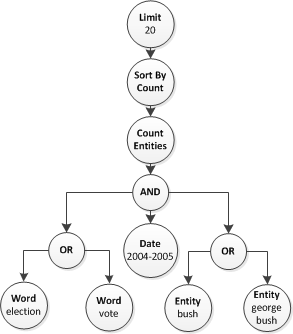
\includegraphics[width=40mm]{figures/entity-query.png}
  }
  \caption{An example query that returns the top 20 entities referenced in articles that mention the election of George Bush.}
  \label{fig:entity-query}
\end{figure}

Queries that return quantitative results, such as document hit counts, request a complete data matrix in a single request.  This minimizes overhead due to network latency and the limited number of simultaneous connections provided by a web-browser.  As shown in figure \ref{fig:json-query}, the queries have three main parameters: a global filter expression, an array of expressions to aggregate separately, and an array of buckets that filter documents into horizontal axis segments.

\begin{figure}[htb]
  \centerline{
    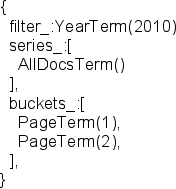
\includegraphics[width=40mm]{figures/json-query.png}
  }
  \caption{An example query expression in 'JSON' using some syntactic sugar functions.}
  \label{fig:json-query}
\end{figure}

The query engine is built in Java using the Jersey RESTful web service framework.  Combining this framework with the Jackson JSON Processor allows for the automatic mapping of HTTP requests with a JSON payload into Java method calls that take Java objects as arguments.  This makes it very easy to build structured query expressions in Javascript and have them processed by the query service.

The query process runs in several phases, figures \ref{fig:query}, \ref{fig:pull}.  First all the input expressions are scanned and validated.  Once the query expression is validated, the series expressions that were submitted are crossed with the requested aggregation buckets to produce a family of query expressions.  Each one is submitted to the evaluator, which checks to see if it has recently processed any similar sub-expressions. If possible it reuses old results as it aggregates the results recursively.  Once the evaluator finishes, the specific logic for the query type applies any additional data transformations required by the front end, e.g. loading the article metadata for matching documents.

\begin{figure}[htb]
  \centerline{
    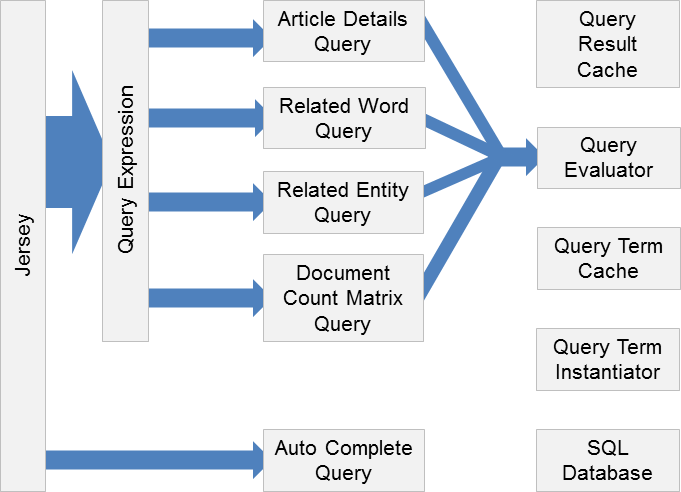
\includegraphics[width=60mm]{figures/query.png}
  }
  \caption{The four main query types are handled by the same query evaluator.}
  \label{fig:query}
\end{figure}

\begin{figure}[htb]
  \centerline{
    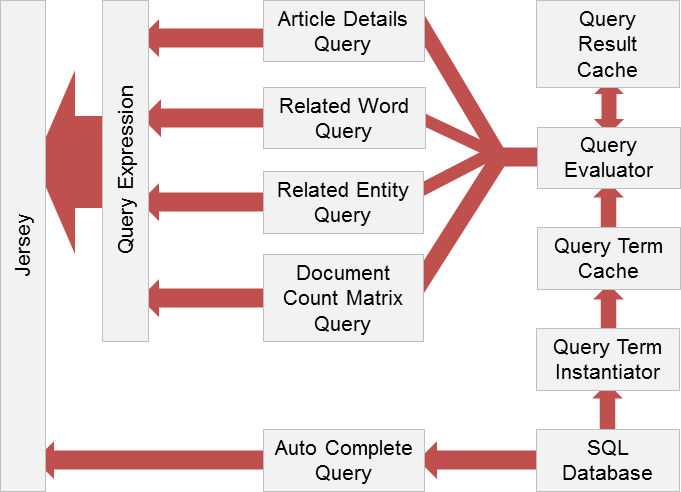
\includegraphics[width=60mm]{figures/pull.png}
  }
  \caption{The query evaluator pulls information from the SQL databasse into in memory caches and temporarily caches intermediate results to maximize interactivity.}
  \label{fig:pull}
\end{figure}


Terminal nodes imply a specific collection of documents, so the engine caches that intermediate state in memory using Java soft references.  If a term has not yet been seen, code is executed against the SQL database to generate the needed intermediate state.  Caching the sets of matching documents expressed by individual query terms allows for more interactive performance as queries are modified by the front end.  Typically, a query term will be reused many times as a user investigates a topic.

Some of the terms requires a large amount of data access to compute.  For example, computing the list of top entities over all documents in the corpus requires the entity list from all 2.5 million documents to be aggregated.  All of the database queries that load the entity list are tweaked to maximize the bandwidth that it can read from data.  Assuming there is adequate memory to allow for the database files to be cached in memory, the engine pulls over 2GB/s of data as it computes the results.  This entire query including data load and aggregation takes less than 15 seconds the first time it is executed, but that is still not fast enough for interactive performance.  The engine avoids needing to repeatedly perform similar hard queries by caching the results of each sub-expression that is evaluated.
%!TEX root = p.tex
\section{Explorer   1}


\begin{figure}[htb]
  \centerline{
    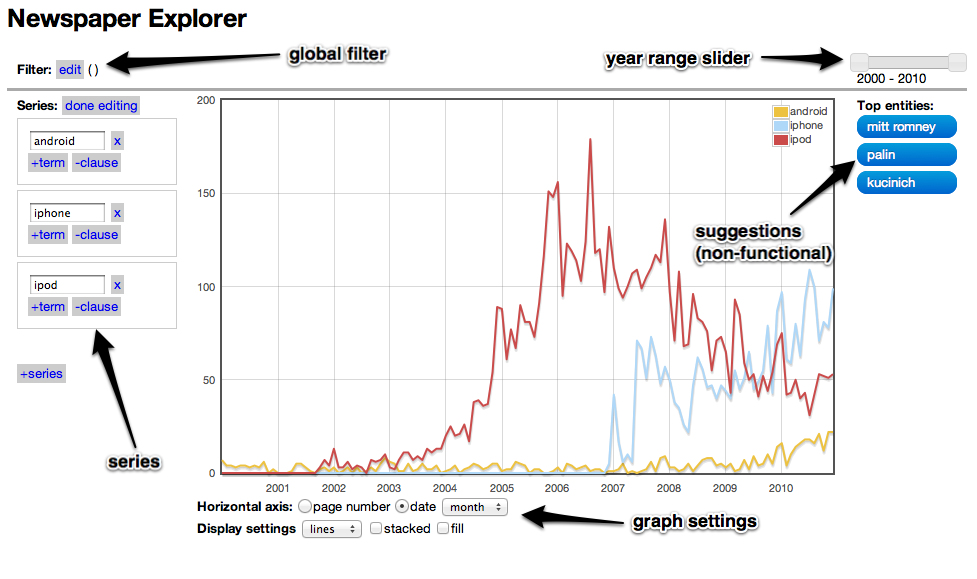
\includegraphics[scale=0.28]{figures/explorer-prototype.png}
  }
  \caption{TODO: FILL ME IN}
  \label{fig:explorer-prototype}
\end{figure}

The first iteration of the �Explorer� interface was designed to allow the visualization of the number of articles containing a given term, bucketed either by time or article page number. It borrowed the concept of �series� from Excel and other familiar charting tools, but allowed the specification of series as unions of the sets of documents containing specified words. For instance, a series like �dog OR cat� could be specified, and the series plotted would represent the number of documents containing one or both of these words. Additionally, this version allowed the user to specify a global filter, which would restrict the view to include only articles that match the series queries as well as the filter query. For instance, if one were to use �pet� as the filter and �dog� and �cat� as series, the two plot lines would represent the result of running queries for �pet AND dog� and �pet AND cat.� The version allowed the specification of arbitrary conjunctive normal form expressions for the filter. Beyond the series and filter features, this first iteration included a number of other features that are self-explanatory, including a year slider, numerous selection widgets for graph settings. 
%!TEX root = p.tex
\section{Entity 1.1}

\begin{figure}[htb]
  \centerline{
    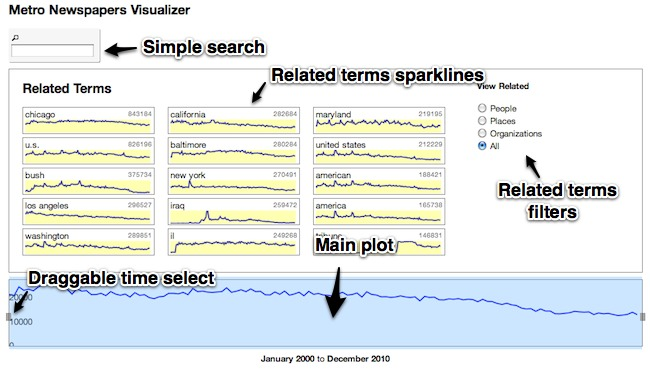
\includegraphics[scale=0.37]{figures/relation-0.jpg}
  }
  \caption{Entity Version 1}
  \label{fig:explorer-0}
\end{figure}

The first iteration of the entity relation viewer was designed to allow the user to quickly navigate between terms and entities related to a base query. Similar to how a user of wikipedia will follow links between related articles and discover new material, users of the entity relation viewer can quickly jump from topic to topic in search of a hidden story buried in the data. This visualization was motivated by our interviews in which users expressed the desire to uncover unexpected relationships and trends in the data.

The viewer consists of a search box where a user can enter a search box, and a large sparkline plot at the bottom which shows the number of articles containing that term through time. About the large sparkline is a list of the top 15 related entities which co-occur in articles with the search term. In addition, each entity is accompanied by a small sparkline with a preview of that entity's trend over time to help the user pick out other interesting trends at a glance.

\section{Entity 1.2}


\begin{figure}[htb]
  \centerline{
    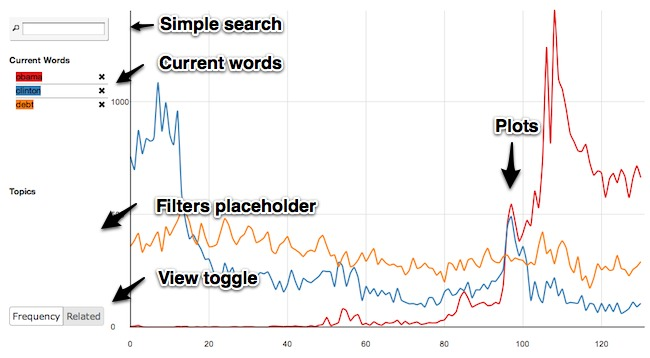
\includegraphics[scale=0.37]{figures/relation-1-a.jpg}
  }
  \caption{Entity Version 2, View 1}
  \label{fig:explorer-1-a}
\end{figure}

The second version of the entity relation viewer prototype was designed with many of the design decisions as the first version. Again quick exploration of related terms and a simple query  methodology were the heart of the design. This prototype does differ from the first version in one major way. In particular it allows frequency comparisons between different terms and assumes this will be at least as useful of an exploration method. As such it allows people to explore the data in two ways; one for related terms and one for frequency comparisons.


\begin{figure}[htb]
  \centerline{
    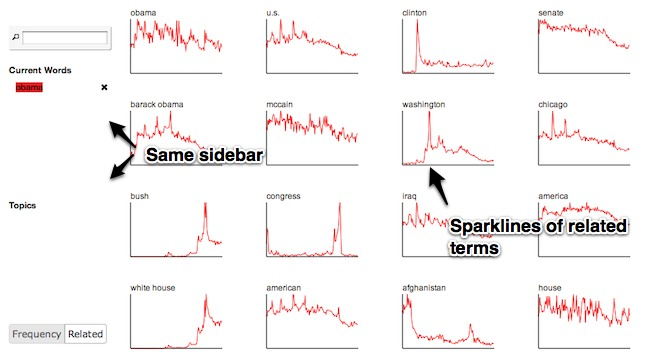
\includegraphics[scale=0.37]{figures/relation-1-b.jpg}
  }
  \caption{Entity Version 2, View 2}
  \label{fig:explorer-1-b}
\end{figure}

%!TEX root = p.tex
\section{Final Designs}
After finishing our three prototypes, we sought feedback from several journalists and researchers, and iterated on our original designs. 

%!TEX root = p.tex
\section{Explorer 2}
Lorem ipsum dolor...


%!TEX root = p.tex
\section{Entity 2}

The second prototype generally received positive feedback. One of the common themes of the demos was that users liked the ability to drill down in the explorer prototype, but liked the simplicity of the entity prototype. Ultimately it seemed like we needed to add the ability to drill down further in to the newspaper data.

We decided the best way to do this, while maintaining ease of use, was to link search terms with the related terms a user clicks. That is if the user searched 'Obama' and clicked the 'Chicago' related term, then both related terms and the main plot would update with articles containing 'Obama' and 'Chicago'. We also had a breadcrumb to handle adding these additional filters. However, after a few extra filters, it wasn't uncommon for only a small number of articles to remain. In addition, this broke the free-form linking from term to term idea so we ultimately removed this feature.

Beyond this issue, there were a number of other things we needed to change after receiving feedback.

\textbf{The ability to drill down to the individual article level was a common request.} This actually came up in our initial interviews with journalists to understand the space as well. To address this, we added mouse over listeners on the main plot to open a dialog with appropriate article titles for the selected time.

\textbf{Testers complained of unintuitive relationships between the sections of the visualization.} Users were not sure whether the time slider in the main dialog affected the related term sparklines and seemed to think that the related term sparklines were the primary feature of the visualization. To address this, we placed the main sparkline above the related terms and made it larger.

\textbf{A few users wanted to see specifically related people to a given person or event}. To address this we added a radio switch to see only related people, places, organizations, or all 3.

\textbf{Several users were confused about how the time slider on the main sparkline related to the related term sparklines.} To address this, we added a highlight to the small sparklines showing here the currently selected timespan falls. 

\textbf{Several users suggested we add instructions.} Because we did not want to take up much space with these instructions we added an information button in the top right of the visualization that has a pop up instructions dialog.

\textbf{The ability to share views of the prototype seemed important to users.} Consequently we added a dynamic URL feature that allows sharing via URL.

The second version of the entity relation viewer, shown in \ref{explorer-1-b}, was discontinued. Though it received decent feedback, it was a difficult prototype to expand in the ways that we wanted to. In particular it was difficult to add query power, and maintain continuity between its two views. In addition, frequency comparisons did not seem as useful as we first suspected. After stopping its development, we focused on the first version of the visualization described above.

\begin{figure}[htb]
  \centerline{
    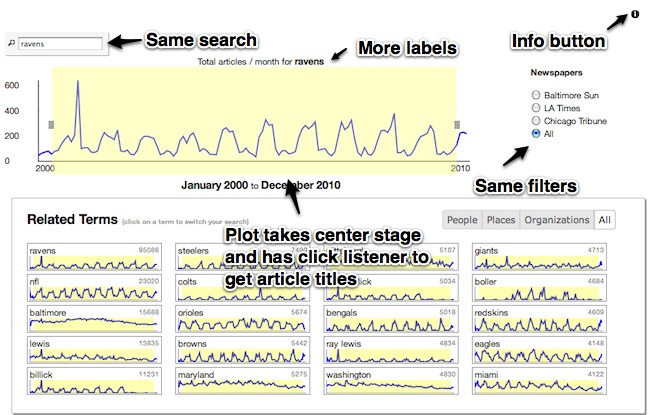
\includegraphics[scale=0.37]{figures/finalTe.jpg}
  }
  \caption{Final version of the entity explorer}
  \label{fig:explorer-1}
\end{figure}


%!TEX root = p.tex
\section{Future}
Lorem ipsum dolor...



\bibliographystyle{abbrv} % 1p
\bibliography{p}

\end{document}
